% !TEX root = ../MasterThesis_Onoe.tex
% 上記はただのコメントではなく親ファイルの場所を教えているので
% 消してしまうとファイルごとのタイプセットができなくなるので注意。
% 親ファイル名を変更したときはここも変更する。

\chapter{ビームテストによる評価実験} \label{sec:Beamtest}
これまでに作成されたSiW-ECALの技術プロトタイプ(FEVおよびCOB)の性能評価実験を、2023年6月7日から2023年6月22日の期間にCERN SPS加速器のビームラインにて行った。本実験の主な目的は、電磁カロリメータとハドロンカロリメータの技術プロトタイプを同じビーム軸上に設置し、同時に運転を行いデータを取得すること。また、これまでの評価実験の中でも最高エネルギーのハドロンビームを用いて15層のSiW-ECALの評価を行うことの2点であった。また本実験におけるハドロンカロリメータは、同じくCALICEグループにおいてドイツやチェコが中心となって開発を進めているAHCALを用いた。以下では実験の詳細と、結果について述べる。
\section{ビームライン}
ビームテストは、フランスとスイスの国境付近に位置する欧州原子核研究機構 (CERN) の、SPS (Super Proton Synchrotron) 加速器のビームラインを用いて行った。SPSは、現在LHC (Large Hadron Collider) の前段加速器として利用されており、陽子シンクロトロンから来た26$\mathrm{GeV}$の陽子を、周長7kmの加速器によって$400\sim 450 \mathrm{GeV}$まで加速している。SPSのビームラインでは、加速した陽子ビームに対してターゲットを用いることで、電子、ミューオン/パイ中間子の2次ビームを運動量$10\sim 400 \mathrm{GeV}$で得ることができる。本実験ではこれらのビームを用いて、NorthエリアにあるH2Aビームラインで実験を行った。実験に用いたビームパラメータを表\ref{beamparam}に示す。\\
\begin{figure}[H]
	\begin{center}
 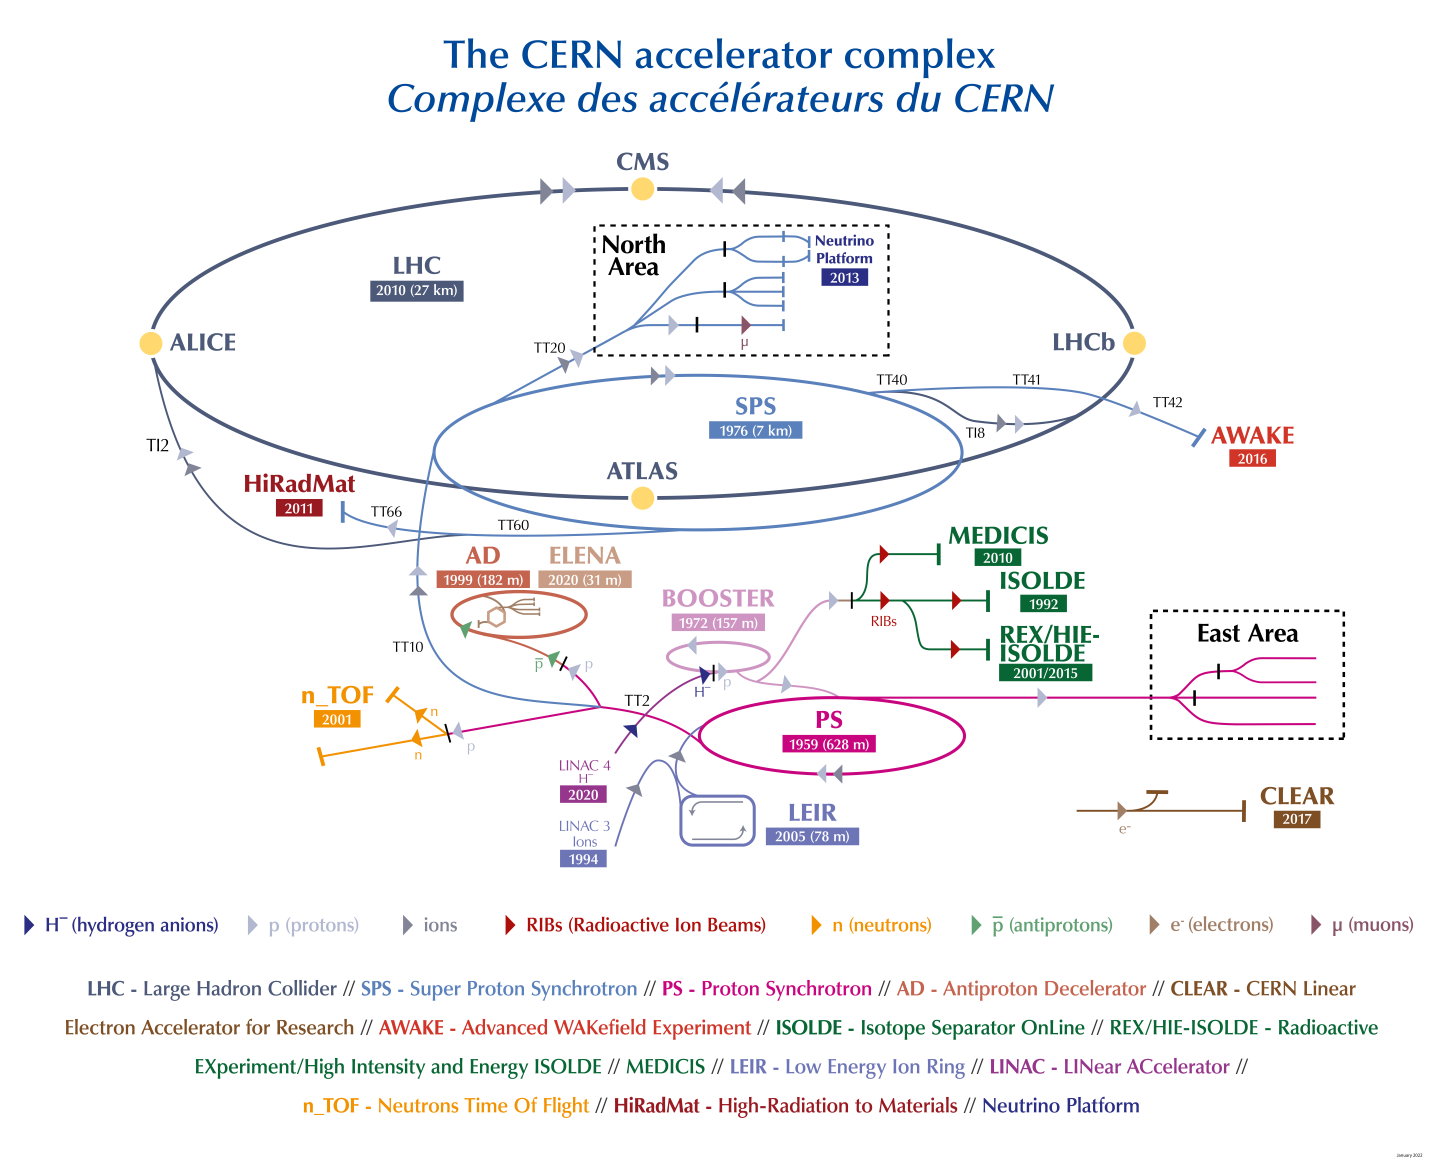
\includegraphics[keepaspectratio, scale=0.7]
 	{Figure/Beamtest/cern.png}
 		\caption{CERNの全体図}
	\end{center}
\end{figure}
\begin{table}[H]
 \centering
 \begin{tabular}{c c}
 \hline
Momentum range & 10-200$[ \mathrm{GeV}/ c ]$\\
Electron purity & 10-99.5\%\\
Max $\delta p / p$  & $2\%$\\
Beam height from floor & 2460$[ \mathrm{mm}]$\\
 \hline
 \end{tabular}
 \label{layer}
 \caption{}
\end{table}

\section{実験セットアップ}
\subsection{測定機器のセットアップ}
本実験でのセットアップの概観を図\ref{setup1}に示す。図中右手からビームが照射され、ILDの構成と同様に上流側にSiW-ECALが、下流側にAHCALを設置した。本論文ではAHCALの解析結果については触れないため、説明を省略する。一方でSiW-ECALのプロトタイプは、FEVを13層(うちFEV11が)COBを2層組み合わせた計15層からなる検出層と鉛板15層の吸収層からなるモジュールを組み立てた。今回のビームテストの検出層は、最も良い性能が期待できるFEV13を前方に設置し、性能比較のためにCOBを加えた構成となった。15層の検出層において、センサーと読み出しボードに供給する電源は、15層に対して図\ref{setup2}左のように並列で印加した。また、信号はカプトンケーブルを通して15層分の信号を一括してCOREモジュールに送り、PCで読み出しを行った。\\
\begin{figure}[H]
\begin{center}
 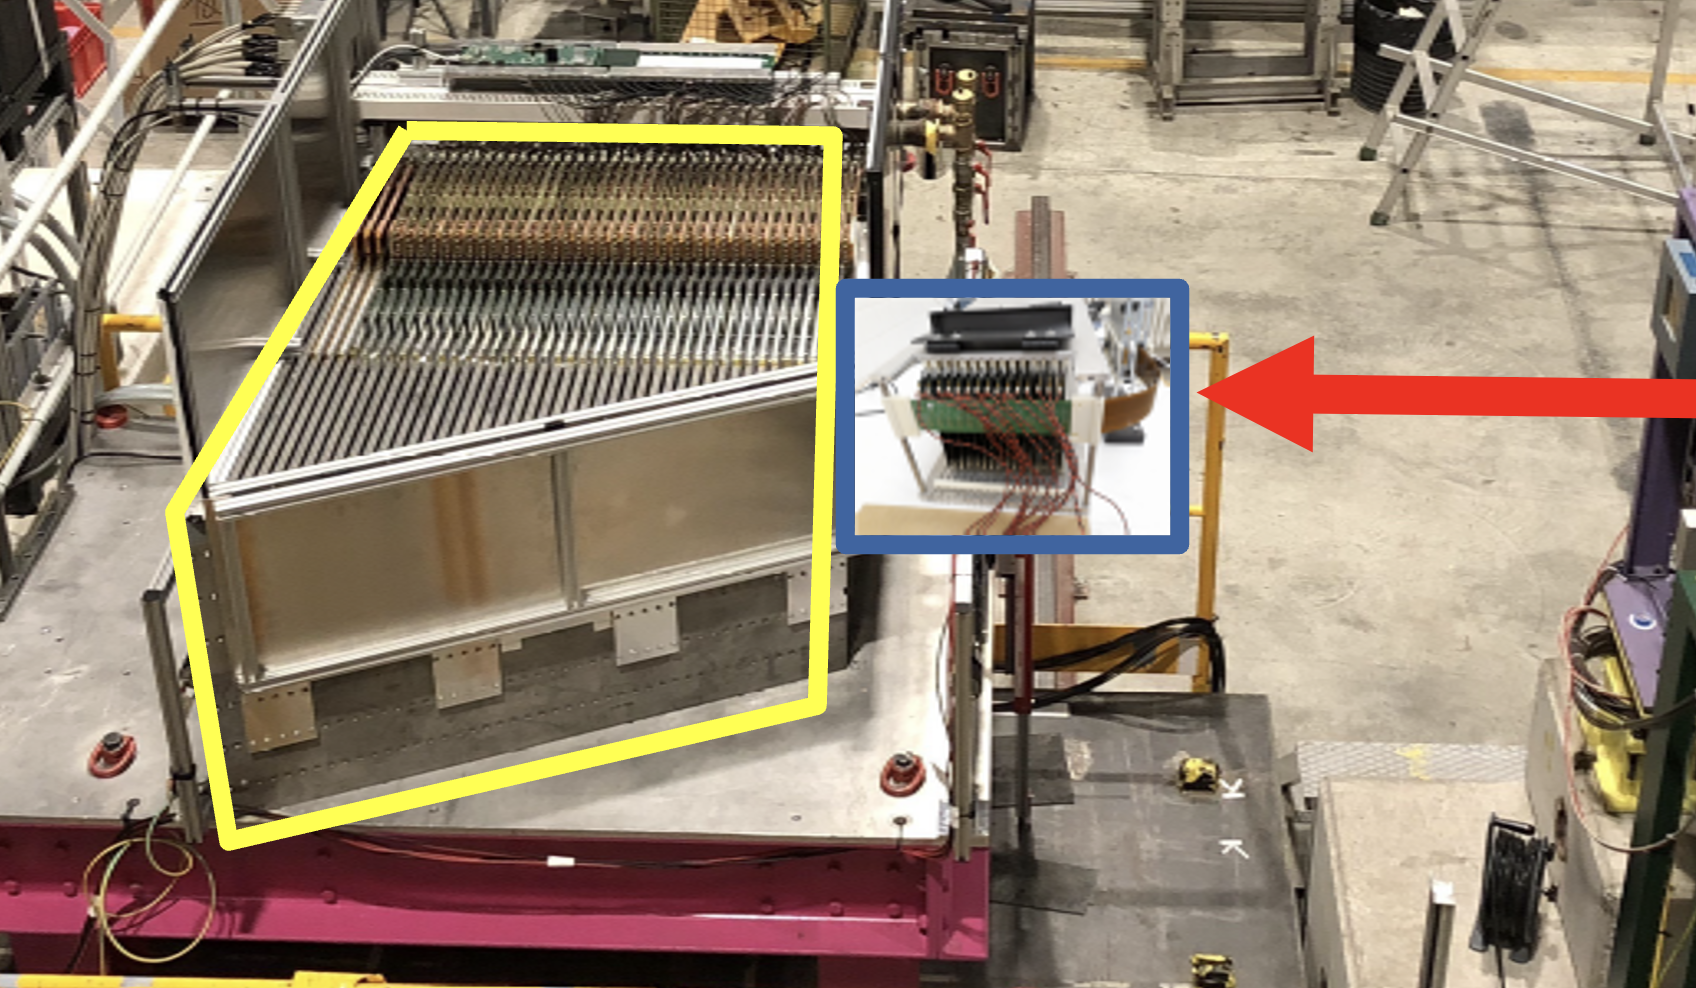
\includegraphics[keepaspectratio, scale=0.3]
 	{Figure/Beamtest/setup1.png}
 		\caption{セットアップの全体図。黄枠:AHCAL、青枠:SiW-ECAL、赤:ビーム位置}
		\label{setup1}
		\end{center}
\end{figure}

\begin{figure}[H]
\begin{center}
 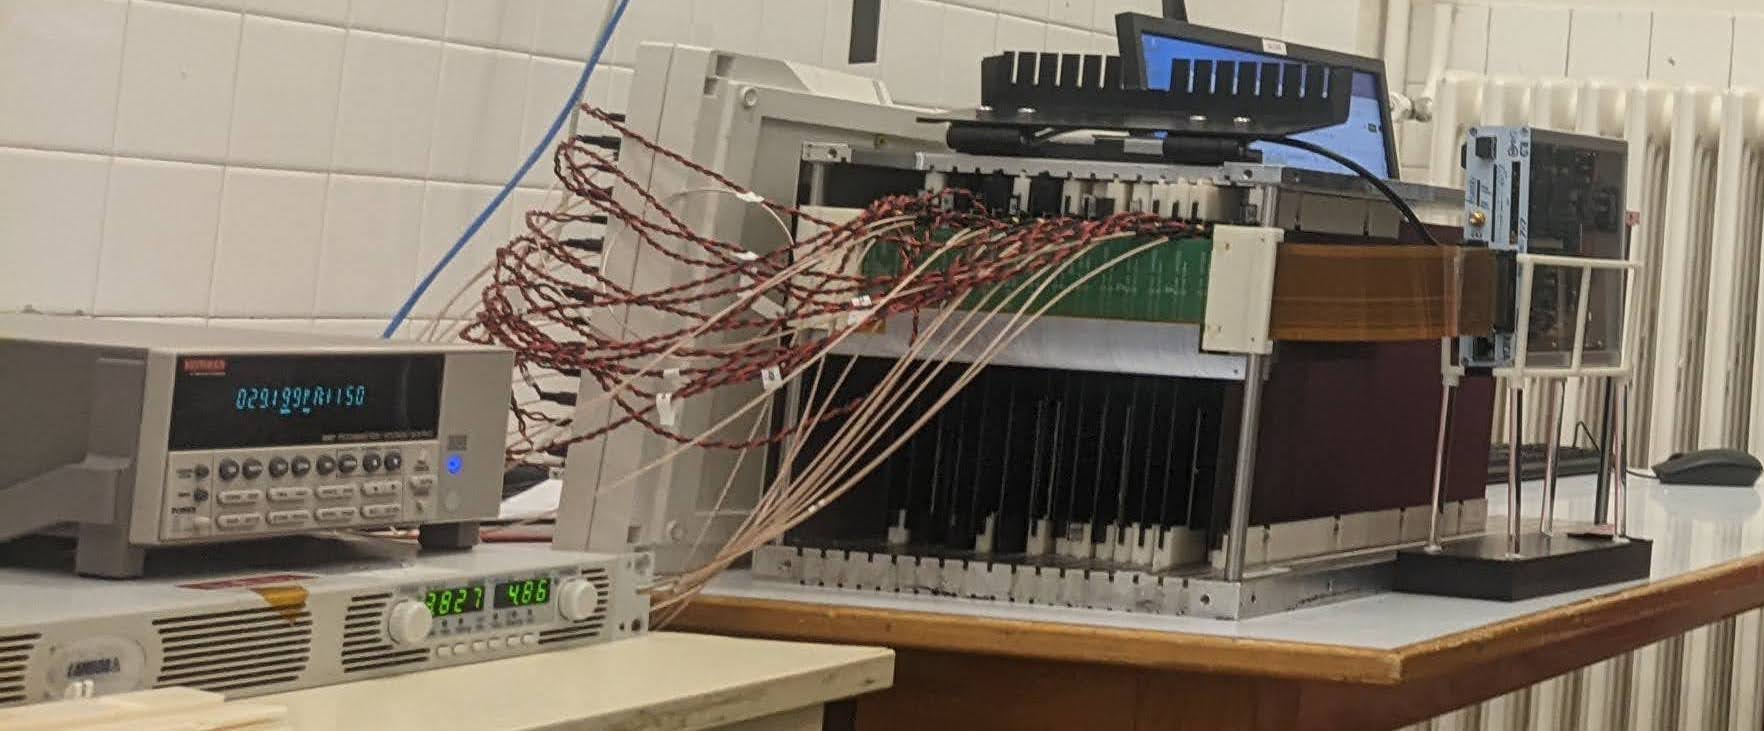
\includegraphics[keepaspectratio, scale=0.2]
 	{Figure/Beamtest/setup2.png}
 		\caption{SiW-ECALのプロトタイプモジュールと電源供給、読み出しシステム}
		\label{setup2}
\end{center}
\end{figure}

\begin{table}[H]
 \centering
 \begin{tabular}{|c|c|c|c|}
 \hline
層数 & ボードの種類 & ウェハー厚み$[\mu m]$ & タングステン厚み[mm]\\
 \hline
 \hline
0 & FEV13 & 650 & 4.2\\
1 & FEV13 & 650 & 4.2\\
2 & FEV13 & 650 & 4.2\\
3 & FEV13 & 650 & 4.2\\
4 & FEV13 & 500 & 4.2\\
5 & FEV13 & 500 & 4.2\\
6 & COB & 500 & 4.2\\
7 & FEV12 & 500 & 4.2\\
8 & COB & 500 & 5.6\\
9 & FEV12 & 500 & 5.6\\
10 & FEV11 & 320 & 5.6\\
11 & FEV11 & 320 & 5.6\\
12 & FEV10 & 320 & 5.6\\
13 & FEV13 & 320 & 5.6\\
14 & FEV11 & 320 & 5.6\\
 \hline
 \end{tabular}
 \label{layer}
 \caption{SiW-ECALのレイヤー構成 (0層目がビーム上流側) }
\end{table}
\subsection{信号読み出し}
ECALとHCALは独立にDAQを行うが、本実験ではEUDAQという読み出しフレームワークによってHCALと同期した読み出しを行った。EUDAQでは、ECALとHCALの間でCCC (Clock and Control Card) を同期させており、CCCではクロック、スタート、ストップ信号をPCへ送っているため、PC上で同じBCIDのイベントを収集することができる。\\
また、ECALでは専用のDAQソフトウェア\cite{ecalsoft}が存在しており、DAQのみでなくチャンネル単位での閾値の設定やイベントのモニター (図\ref{monitor}) が可能となっている。データはraw形式で保存され、解析用のソフトウェアを通してrootファイルへ変換し解析に利用することができる。
\begin{figure}[H]
\begin{center}
 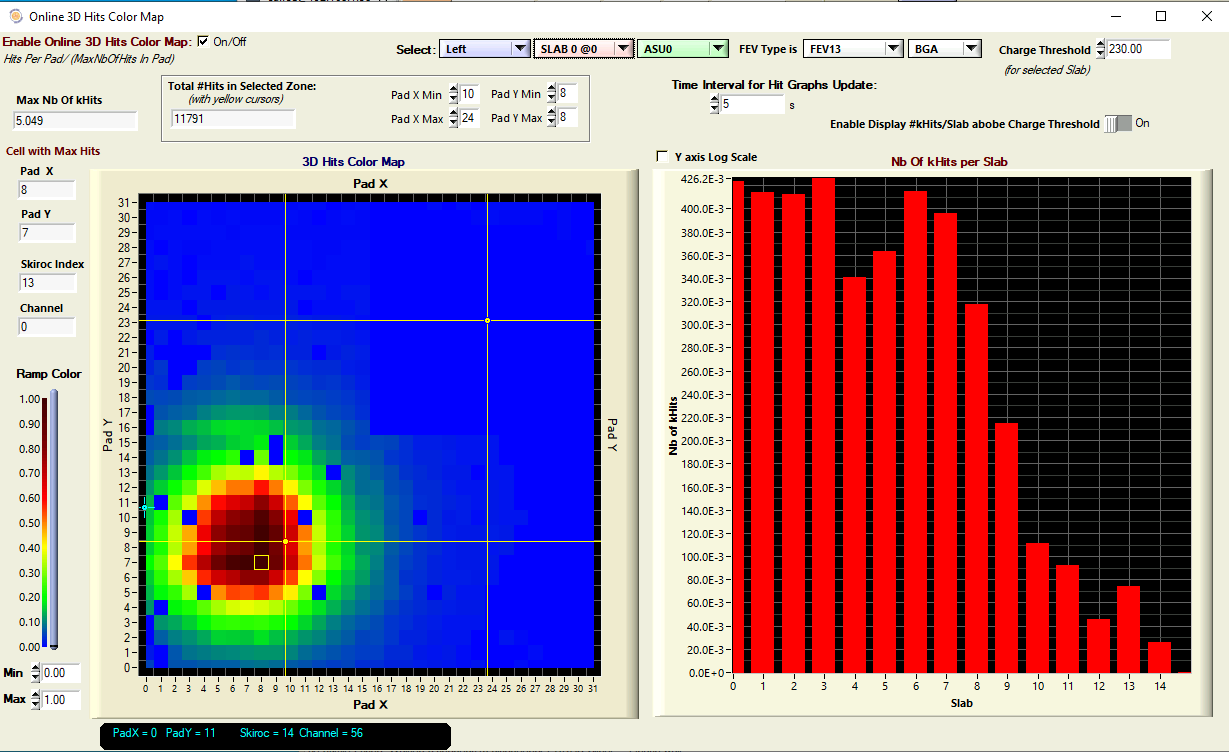
\includegraphics[keepaspectratio, scale=0.2]
 	{Figure/Beamtest/monitor.png}
 		\caption{SiW-ECAL読み出しソフトウェアにおけるイベントモニター (左) ヒットマップ (右) 各層あたりのヒット数}
		\label{monitor}
\end{center}
\end{figure}
\section{実験結果}
\subsection{検出器応答}
各runに対して層ごとのヒットマップを作成し、各層の応答を確認した。作成したヒットマップが図\ref{hitmap}である。ビームはヒットマップ左下のセンサーを中心に照射を行った。\\
電子ビームは相互作用を起こし電磁シャワーを形成するため、ビーム断面積が大きくなっていることが確認できる。またミューオンビームは、電子ビームと比較して相互作用を起こさず、ビームサイズが小さい。また白く抜けている箇所はノイズが多いためマスクしている、あるいは信号がないチャンネルであるが、ビームの種類によらず全体を通して4つほど四角く抜けている部分が確認できる。これは1枚のセンサーの場所と対応しており、実験後に確認したところセンサーとPCBの間の導電性接着剤が剥がれてしまっていることが発覚した。\\
さらにビームのエネルギーを上げていくと、80GeV以上のエネルギーで図\ref{hitmap} (b)第6層のような、1センサー全体にヒットが集中してしまう現象が確認された。エネルギーが大きくなった場合にはセンサーに入ってくる信号が多くなることから、センサー周辺での放電等が原因として考えられるが、現在調査を行なっている。
\begin{figure}[H]
  \begin{minipage}[b]{0.45\linewidth}
    \centering
    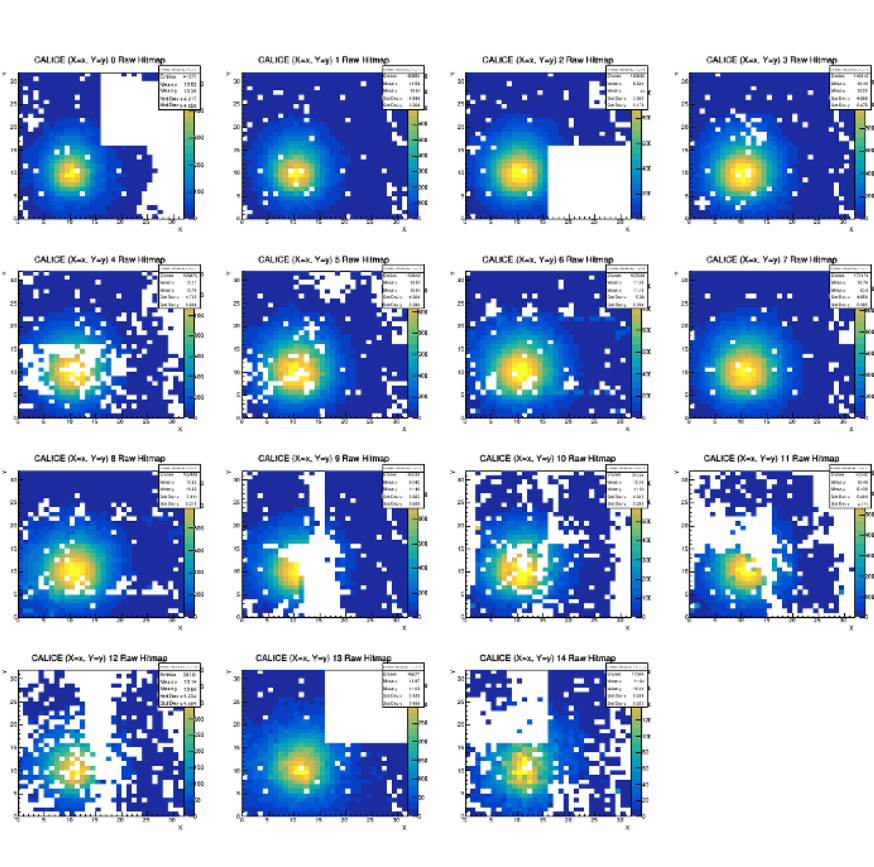
\includegraphics[keepaspectratio, scale=0.2]{Figure/Beamtest/hitmap_e20.png}
    \subcaption{20$\mathrm{GeV}$電子ビーム}
  \end{minipage}
    \begin{minipage}[b]{0.45\linewidth}
    \centering
    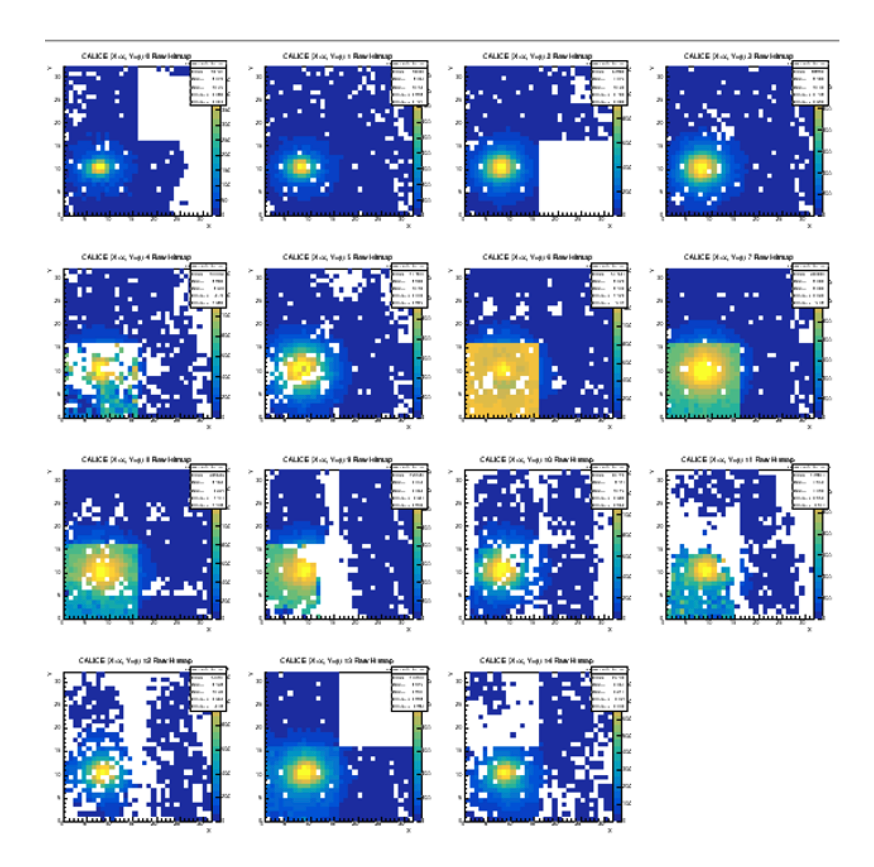
\includegraphics[keepaspectratio, scale=0.2]{Figure/Beamtest/hitmap_e150.png}
    \subcaption{150$\mathrm{GeV}$電子ビーム}
  \end{minipage}
  \begin{minipage}[b]{0.45\linewidth}
    \centering
    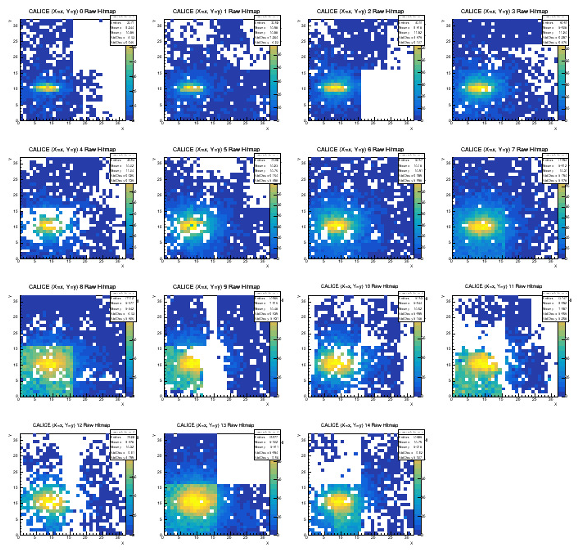
\includegraphics[keepaspectratio, scale=0.2]{Figure/Beamtest/hitmap_mu150.png}
    \subcaption{ミューオンビーム}
   \end{minipage}
   \hfill
  \begin{minipage}[b]{0.45\linewidth}
    \centering
    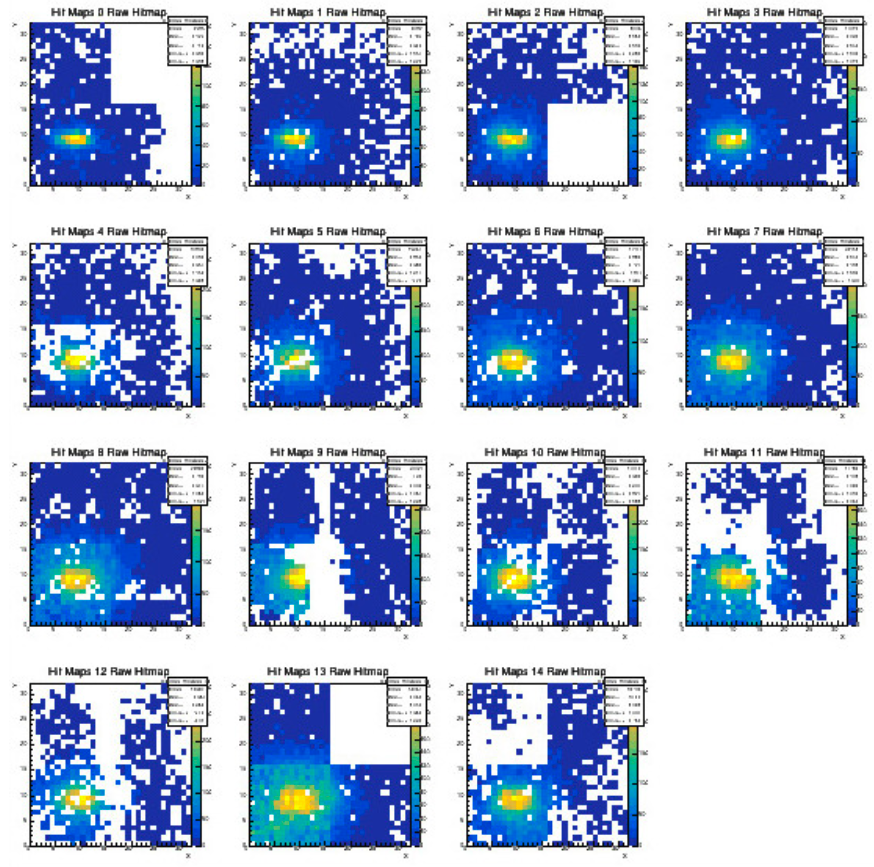
\includegraphics[keepaspectratio, scale=0.2]{Figure/Beamtest/hitmap_pi150.png}
    \subcaption{150$\mathrm{GeV}$パイ中間子ビーム}
  \end{minipage}
  \caption{各ビーム種類におけるヒットマップ。左上から0層右上が3層、右下が14層と順に並んでいる。}
  \label{hitmap}
\end{figure}
\subsection{ペデスタル}
続いて、ペデスタルの解析を行った。ペデスタルとはトリガーが入っていない時の信号の大きさで、エレキ由来のノイズ等によって0でない値を取る。実際のヒットによる信号の大きさは、得られたすべての値からペデスタルの値を引いた値になるため、ペデスタルについて十分に解析を行うことは重要となる。一般的にぺデスタルはガウシアンでフィッティングすることができ、その中央値はペデスタル信号の大きさを、幅はその揺らぎの大きさに相当する。図\ref{pedestal}に各エネルギーの電子ビームのrunにおける同じチャンネルのペデスタルを示した。\\
\begin{figure}[H]
\begin{center}
 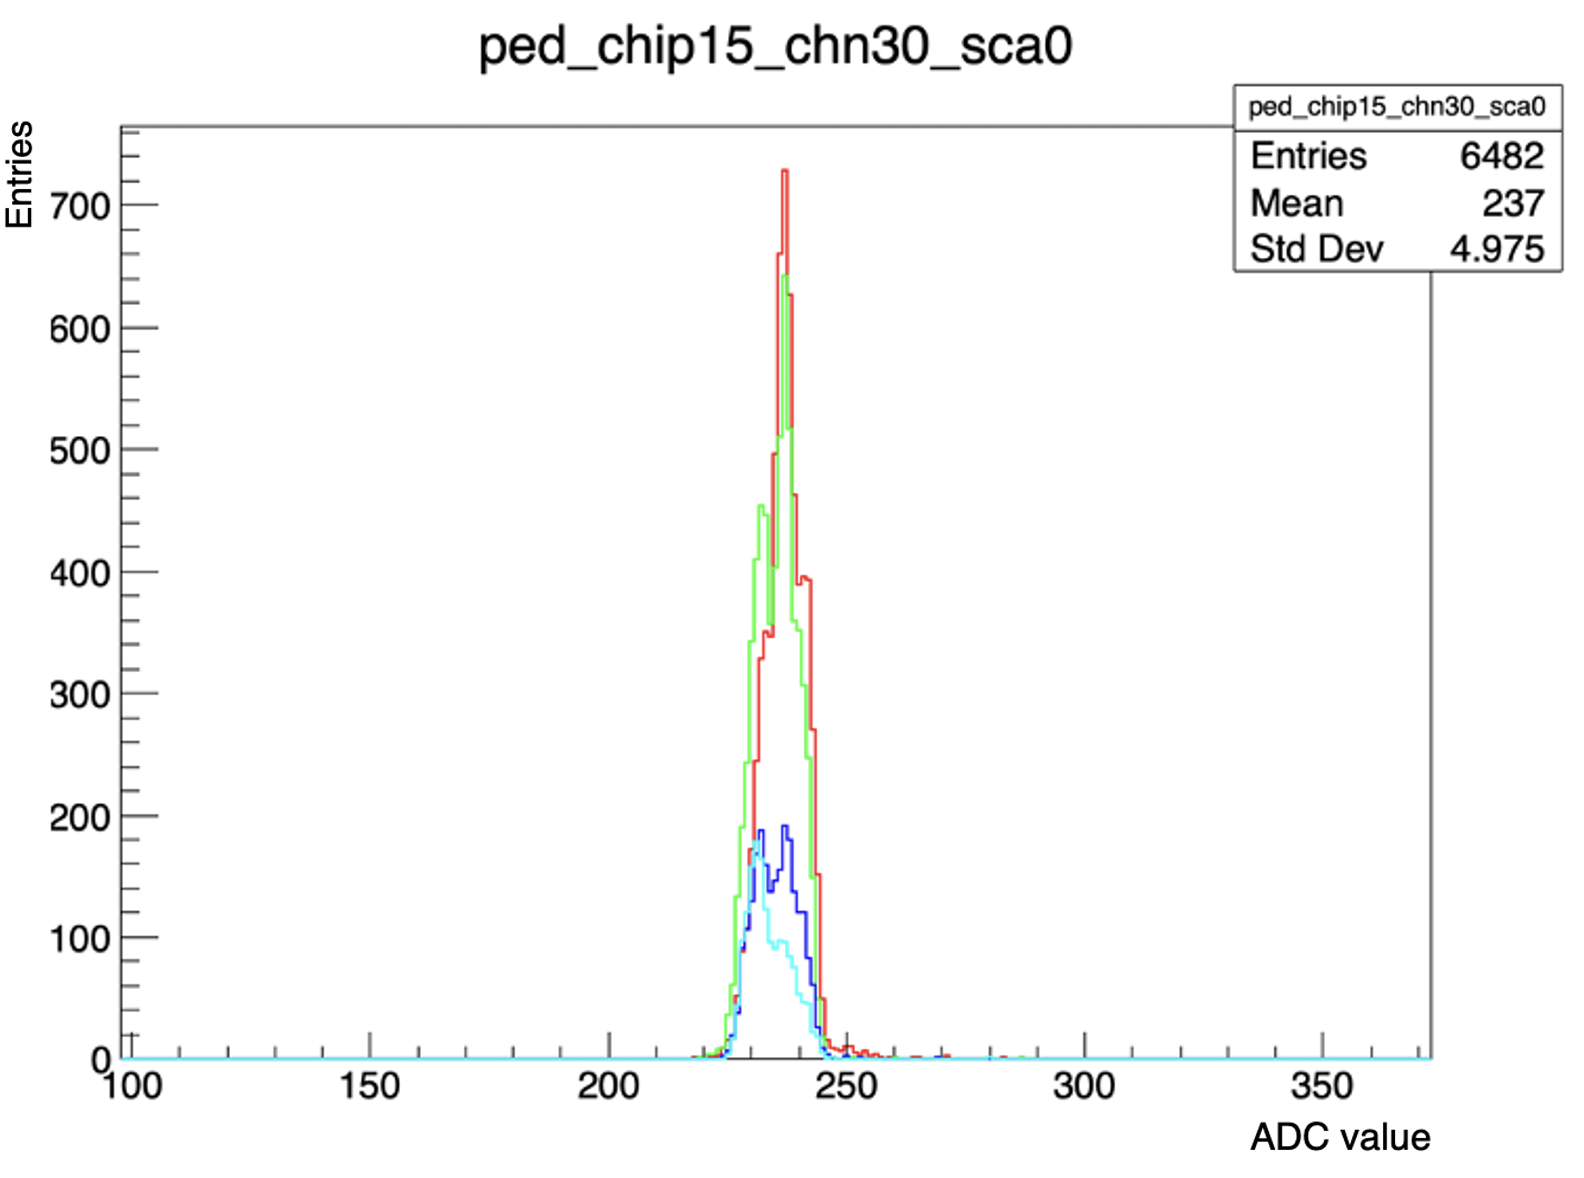
\includegraphics[keepaspectratio, scale=0.5]
 	{Figure/Beamtest/pedestal.png}
 		\caption{40/60/100/150$\mathrm{GeV}$の電子ビームにおけるペデスタル}
		\label{pedestal}
\end{center}
\end{figure}
\begin{figure}[H]
\begin{center}
 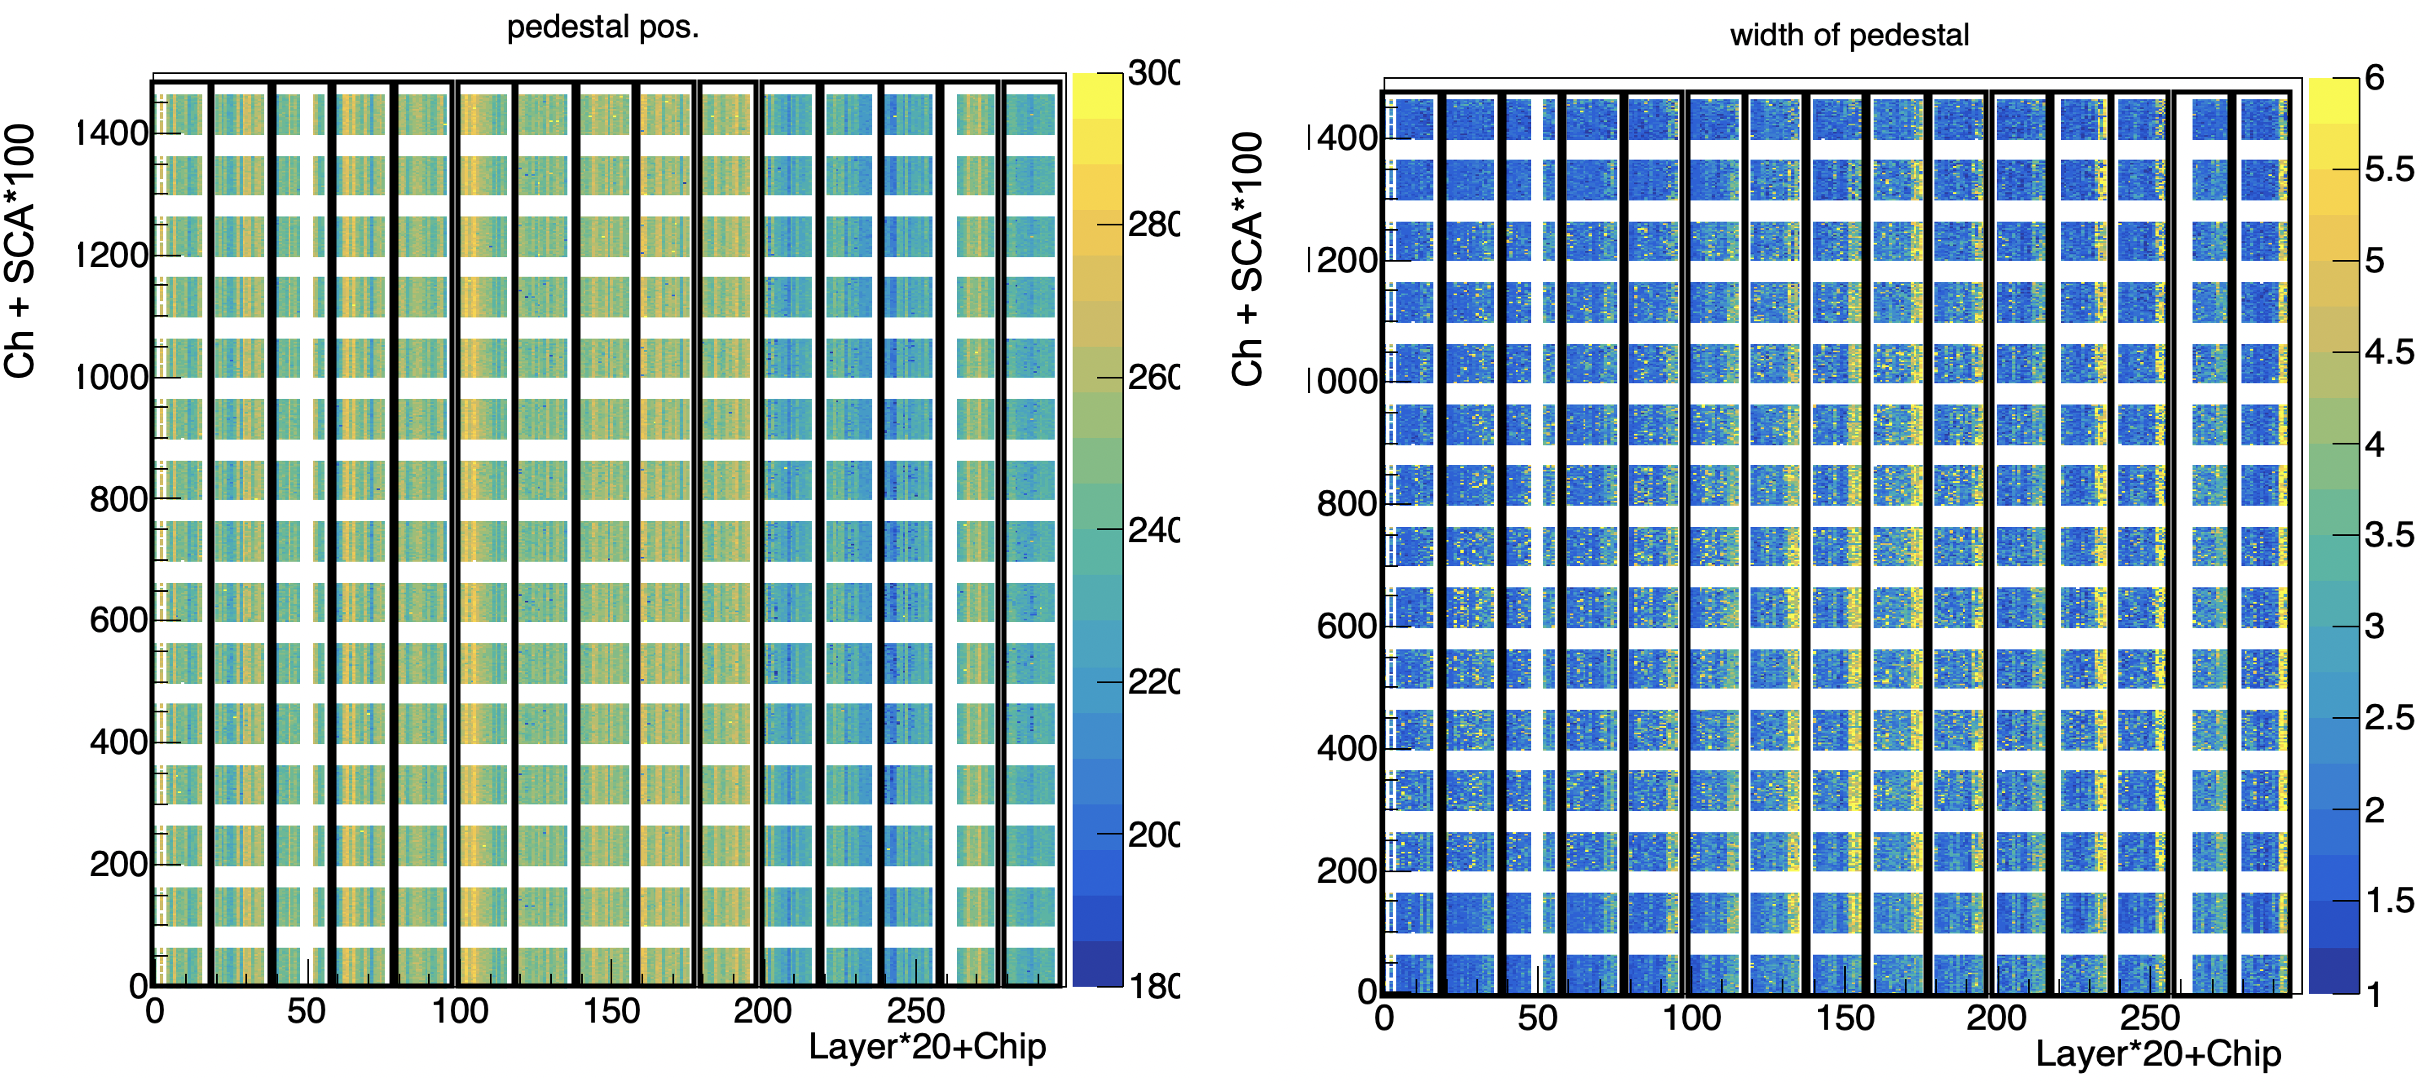
\includegraphics[keepaspectratio, scale=0.3]
 	{Figure/Beamtest/ped_pos.png}
 		\caption{ペデスタルをガウシアンフィットした際のパラメータ。横軸がチップを、縦軸がチャンネル番号を表しており、それぞれ全層、全SCAでの可視化のため、層数やSCAをかけた値となっている。(左) ガウシアンの中央値 (右) ガウシアンの幅の大きさ}
		\label{monitor}
\end{center}
\end{figure}

また、チャンネルによって図\ref{dp}に示すような2つのピークを持つペデスたるが確認された。このペデスタルピークが2つ見える現象をダブルぺデスタルと呼んで調査を行なった。
\begin{figure}[H]
\begin{center}
 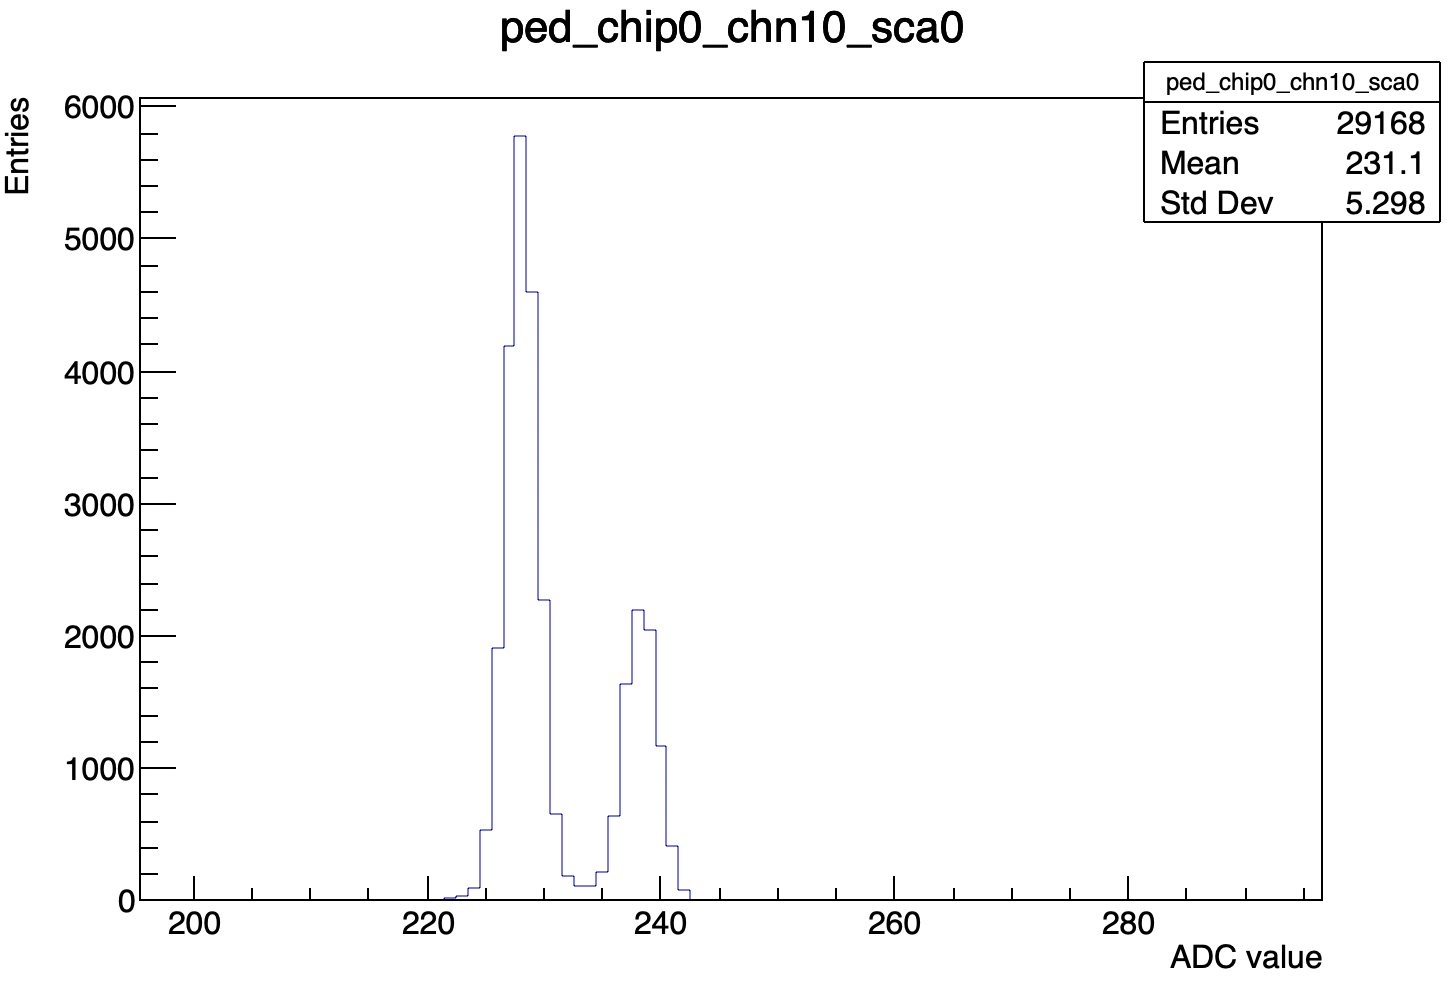
\includegraphics[keepaspectratio, scale=0.5]
 	{Figure/Beamtest/dp.png}
 		\caption{ダブルペデスタルの例}
		\label{dp}
\end{center}
\end{figure}
%\subsection{スクエアイベント}
\section{まとめと考察}
記入予定
(メモ:各Slabは実験前にモジュールへのインストールと動作確認を行い、緩衝材で梱包して輸送した。)